\chapter{Introduction}
\paragraph*{}
Life needs energy to continue its spread. Plants use photosynthesis to separate carbon from oxygen and to grow. Higher life forms as humans consume energy during the day and during the night, being dependent on the available energy source~\cite{energy_consumption_review}. While fossil fuels are still the major source of energy~\cite{energy_sources_review} and while fire is used to convert the Joules that hold together hydrocarbon molecules into a "horse power" of a combustion engine and kilowatt-hours in a power socket, there are cleaner and more efficient ways to harvest energy. Photosynthesis had inspired the creation of solar panels that convert the sunlight into electricity, the atom had been tamed in the core of a nuclear reactor to power cities; we can extract energy from sound~\cite{energy_from_sound}, wind and waves and from the heat of the planet. Moreover, there are hopes and continuous attempts to achieve nuclear fusion~\cite{tokamak_updates} - the creation of an artificial Sun by melting together atomic cores - the virtually inexhaustible and clean source of energy. The oil and gas are limited and unevenly distributed resources, wind does not always blow, the Sun does not shine at night, the wild Nature is still unpredictable and the extracted energy has to be stored in order to level out its production and consumption.\\
\paragraph*{}
With the rise of the technological era, over the last century, energy has been delivered to our homes in form of electricity. The storage of electrical energy is the key ingredient of every power grid, every electrical device. Electric charges separated by a potential barrier can store energy in a device called a battery, or, precisely, a battery of electrochemical cells. It is also possible to store energy in an electrostatic field between the plates of a capacitor\cite{supercaps_review}, but due to the technological difficulties, electrochemical cells are commonly used instead. An electrochemical cell is an energy storage device that undergoes a chemical reaction to release electrical energy. A simple electrochemical cell consists of two spatially separated materials called electrodes, that have different work functions, or, chemically speaking, reduction-oxidation (redox) potentials. The electrodes are separated with a layer of ions that allow for the transfer of charge between the electrodes when they are connected to each other with a conductor. The conductor passes the electric current through an electric circuit and powers it. While the battery delivers the electric current to the circuit, a chemical reaction is happening on its electrodes: the positively charged electrode, called cathode, is being reduced, obtaining electrons from the negatively charged anode through the conductor. The anode loses electrons and is being oxidized. The speed, reversibility, released by-products and physical conditions of this redox reaction are the key factors that define the performance of an electrochemical cell. This reaction had been of great interest for the field of energy storage, particularly, electrochemistry, where numerous characterization techniques have been developed to optimize the architecture of batteries.\\
\paragraph*{}
Stable, capacious and powerful batteries have become of great demand for today's energy driven society~\cite{Yoo2014,Xu2020,Nitta2015}. The advances in lithium ion technology for rechargeable batteries have enabled energy densities that make it possible to battery-power a wearable Internet-of-things device~\cite{Lee2013,Maddikunta2020}, an airplane~\cite{Kadlec2014} or a house~\cite{Diouf2019,Hirasawa2021}. Still, the application of lithium ion batteries is limited by irreversible processes~\cite{Larsson2017,Fu2015,Zhang2021} that occur upon extreme operating conditions such as high power demand~\cite{Zhang2022,Guan2018} or over-discharge~\cite{Ma2020}. Such degradation processes limit the performance of a battery by lowering its safe operating power, resulting in lower power density and longer charging times. The challenge to overcome these limitations, together with low abundance of the rare earth metals~\cite{Xu2020} and the toxicity of the manufacturing process~\cite{Prazanov2022,Peters2017} is motivating research and development of advanced battery technologies~\cite{Degen2022}. This requires understanding of charge transport and degradation pathways in energy storage materials as well as exploring novel materials such as materials based on organic precursors~\cite{Lu2020,Kim2023}.
\paragraph*{}
Organic radical batteries (ORB) based on redox polymers containing stable radicals~\cite{nakahara2002_cpl} have been shown to compete with or even outperform  conventional Li based batteries in terms of power densities~\cite{IWASA2007} with the additional benefit of being free from rare precursors, inheriting mechanical properties of plastics and electrical properties of semiconductors~\cite{friebe2017_topcurrchem,Casado2021,Goujon2021}. Advanced molecular design techniques allow for tuning of the electrochemical properties of the redox polymers~\cite{Janoschka2017}, that brings in a rich variety of organic energy storage materials~\cite{Xie2021,Vereshchagin2022,Janoschka2017a} and creates a large room for their optimization. 
\paragraph*{}
Redox conductive conjugated polymers containing TEMPO (2,2,6,6-tetramethylpiperidine-1-oxyl) redox groups, as pDiTBuS (poly-di-TEMPO-Butyl-Salen) shown in Figure~\ref{fig:Figure_1}, demonstrate particularly promising energy and power densities~\cite{Vereshchagin2020}. The pDiTBuS was designed as a cathode material: it is oxidized when the electrochemical cell containing this material is charged. A film of pDiTBuS comprises a high concentration of redox active stable nitroxyl radicals attached to a conjugated polymer backbone that interconnects them as a molecular wire. Such system may be viewed as a highly disordered molecular hole-transporting semiconductor (the poly-NiSalen backbone) that contains a large amount of hole traps (TEMPO groups) attached to it with butyl linkers. When the film is reduced (discharged), the TEMPO groups are in the radical state and act as unfilled traps. Upon oxidation (charging), the TEMPO fragments lose an unpaired electron and acquire a positive charge, so the traps are being filled with holes.

\begin{figure}[h]
\center
	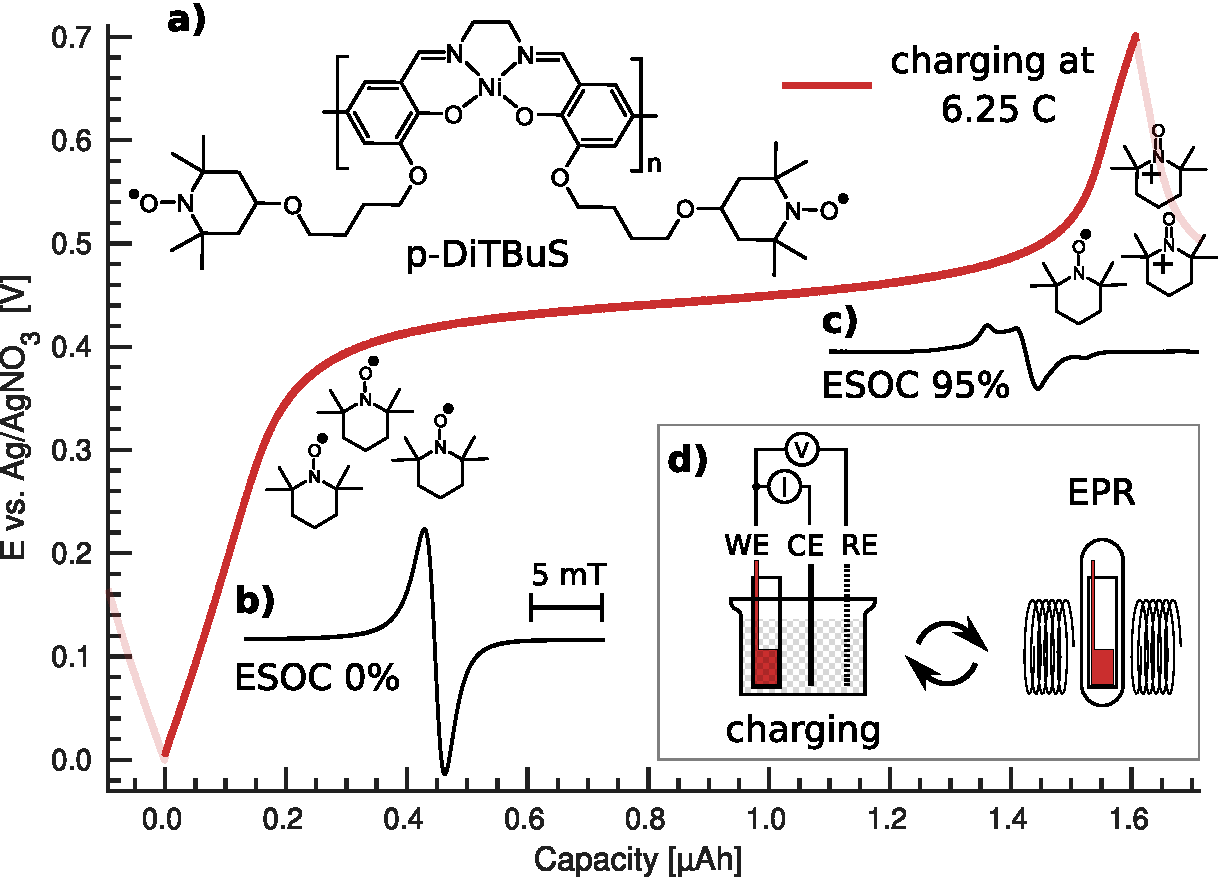
\includegraphics[width=0.7\textwidth]{./introduction/figures/Figure_1.pdf}
	\caption{Galvanostatic charge-discharge curve for a pDiTBuS cathode film at 10~$\muup$A (6.25~C), chemical structure of pDiTBuS (a), normalized cwEPR spectral signatures for reduced (b) and oxidized (c) states. Scheme of the ex-situ EPR measurement on the pDiTBuS half cell (d).}
	\label{fig:Figure_1}
\end{figure}


\paragraph{}
The flexible molecular design together with questions regarding unresolved charge transport- and performance limiting mechanisms have inspired a variety of characterization techniques to be developed and applied to both energy storage materials and energy storage devices, operando and ex-situ. Together with electrochemical characterization as the standard method for studying the properties of energy storage materials\cite{IWASA2007,Zens2022}, operando optical microscopy~\cite{Merryweather2022}, neutron imaging~\cite{Ma2020} and X-ray diffraction~\cite{Rhodes2012} were applied to monitor irreversible structural deformations during extreme charging of Li cells.

UV and IR spectroscopy turned out to be particularly useful for studying organic energy-storage materials. For instance, it was possible to observe formation of positive polarons in the NiSalen backbone of the pDiTBuS upon its oxidation~\cite{Dmitrieva2018}.
Since the electrochemical processes happen within the bulk of the energy storage material and involve changes in the spin states, imaging techniques based on magnetic resonance can be applied to obtain structural information on the battery electrodes on the molecular level~\cite{Niemoller2018,Meier2013,Li2019,Bittl2005}. NMR was used to study dendrite formation, electrolyte dynamics and intercalation of Li ions\cite{Kushida1980,Grosu2023a} in Li cells, including operando imaging~\cite{Shi2019}. 


Operando continuous-wave EPR (cwEPR) was applied to study redox kinetics of inorganic battery cathodes~\cite{Niemoller2019}, radical formation and spin densities in redox polymers~\cite{Dmitrieva2018} and in organic electrochemical cells~\cite{huang2016_jpowersources,Kulikov2022}.

Pulsed EPR (pEPR) provides an even more powerful toolbox for material studies with the electron spin as a microscopic structural probe. In particular, pEPR provides access to the dipolar coupling between neighboring electron spins and thus the possibility to determine distances between adjacent redox-active centers using dipolar spectroscopy~\cite{Salikhov1981} as in spin-labelled proteins~\cite{jeschke2012_annrevphyschem,Toropov1998}. In addition, the hyperfine coupling between electron and nuclear spins in close vicinity can be measured by electron spin echo envelope modulation (ESEEM) and electron nuclear double resonance (ENDOR) techniques and can thus elucidate the degree of delocalization for charge carriers in ORB materials in a similar way as in organic seminconductors~\cite{Behrends2011}.


\paragraph*{}
\raw{EDMR is allowing to manipulate the spin of an electron that tunnels through a disordered media such as the amorphous silicon in a solar cell, through intertwined fragments of conjugated polymers in an organic solar cell or an organic field-effect transistor.}\\




